\documentclass[11pt,a4j, titlepage]{jarticle} %titlepageで表紙のページ番号をなくす
\usepackage[dvipdfmx,dvips]{graphicx}
\usepackage{otf}
\usepackage{amsmath,amssymb}
\usepackage{ascmac,here,txfonts}
\usepackage{listings,jlisting}
\usepackage{color}
\usepackage{epsfig}
\usepackage{fancybox}
\usepackage{epstopdf}
\usepackage{bm}
\usepackage{cases}
\usepackage{comment}
\usepackage{setspace}
\usepackage{subcaption}
\usepackage{array}
\usepackage{enumerate}
\usepackage{url}
%%% jdummy.def
%
\DeclareRelationFont{JY1}{mc}{it}{}{OT1}{cmr}{it}{}
\DeclareRelationFont{JT1}{mc}{it}{}{OT1}{cmr}{it}{}
\DeclareFontShape{JY1}{mc}{m}{it}{<5> <6> <7> <8> <9> <10> sgen*min
    <10.95><12><14.4><17.28><20.74><24.88> min10
    <-> min10}{}
\DeclareFontShape{JT1}{mc}{m}{it}{<5> <6> <7> <8> <9> <10> sgen*tmin
    <10.95><12><14.4><17.28><20.74><24.88> tmin10
    <-> tmin10}{}
\DeclareRelationFont{JY1}{mc}{sl}{}{OT1}{cmr}{sl}{}
\DeclareRelationFont{JT1}{mc}{sl}{}{OT1}{cmr}{sl}{}
\DeclareFontShape{JY1}{mc}{m}{sl}{<5> <6> <7> <8> <9> <10> sgen*min
    <10.95><12><14.4><17.28><20.74><24.88> min10
    <-> min10}{}
\DeclareFontShape{JT1}{mc}{m}{sl}{<5> <6> <7> <8> <9> <10> sgen*tmin
    <10.95><12><14.4><17.28><20.74><24.88> tmin10
    <-> tmin10}{}
\DeclareRelationFont{JY1}{mc}{sc}{}{OT1}{cmr}{sc}{}
\DeclareRelationFont{JT1}{mc}{sc}{}{OT1}{cmr}{sc}{}
\DeclareFontShape{JY1}{mc}{m}{sc}{<5> <6> <7> <8> <9> <10> sgen*min
    <10.95><12><14.4><17.28><20.74><24.88> min10
    <-> min10}{}
\DeclareFontShape{JT1}{mc}{m}{sc}{<5> <6> <7> <8> <9> <10> sgen*tmin
    <10.95><12><14.4><17.28><20.74><24.88> tmin10
    <-> tmin10}{}
\DeclareRelationFont{JY1}{gt}{it}{}{OT1}{cmbx}{it}{}
\DeclareRelationFont{JT1}{gt}{it}{}{OT1}{cmbx}{it}{}
\DeclareFontShape{JY1}{mc}{bx}{it}{<5> <6> <7> <8> <9> <10> sgen*goth
    <10.95><12><14.4><17.28><20.74><24.88> goth10
    <-> goth10}{}
\DeclareFontShape{JT1}{mc}{bx}{it}{<5> <6> <7> <8> <9> <10> sgen*tgoth
    <10.95><12><14.4><17.28><20.74><24.88> tgoth10
    <-> tgoth10}{}
\DeclareRelationFont{JY1}{gt}{sl}{}{OT1}{cmbx}{sl}{}
\DeclareRelationFont{JT1}{gt}{sl}{}{OT1}{cmbx}{sl}{}
\DeclareFontShape{JY1}{mc}{bx}{sl}{<5> <6> <7> <8> <9> <10> sgen*goth
    <10.95><12><14.4><17.28><20.74><24.88> goth10
    <-> goth10}{}
\DeclareFontShape{JT1}{mc}{bx}{sl}{<5> <6> <7> <8> <9> <10> sgen*tgoth
    <10.95><12><14.4><17.28><20.74><24.88> tgoth10
    <-> tgoth10}{}
\DeclareRelationFont{JY1}{gt}{sc}{}{OT1}{cmbx}{sc}{}
\DeclareRelationFont{JT1}{gt}{sc}{}{OT1}{cmbx}{sc}{}
\DeclareFontShape{JY1}{mc}{bx}{sc}{<5> <6> <7> <8> <9> <10> sgen*goth
    <10.95><12><14.4><17.28><20.74><24.88> goth10
    <-> goth10}{}
\DeclareFontShape{JT1}{mc}{bx}{sc}{<5> <6> <7> <8> <9> <10> sgen*tgoth
    <10.95><12><14.4><17.28><20.74><24.88> tgoth10
    <-> tgoth10}{}
\DeclareRelationFont{JY1}{gt}{it}{}{OT1}{cmr}{it}{}
\DeclareRelationFont{JT1}{gt}{it}{}{OT1}{cmr}{it}{}
\DeclareFontShape{JY1}{gt}{m}{it}{<5> <6> <7> <8> <9> <10> sgen*goth
    <10.95><12><14.4><17.28><20.74><24.88> goth10
    <-> goth10}{}
\DeclareFontShape{JT1}{gt}{m}{it}{<5> <6> <7> <8> <9> <10> sgen*tgoth
    <10.95><12><14.4><17.28><20.74><24.88> tgoth10
    <-> tgoth10}{}
\DeclareFontShape{JY1}{mc}{m}{sc}{<5> <6> <7> <8> <9> <10> sgen*min
    <10.95><12><14.4><17.28><20.74><24.88> min10
    <-> min10}{}
\DeclareFontShape{JT1}{mc}{m}{sc}{<5> <6> <7> <8> <9> <10> sgen*tmin
    <10.95><12><14.4><17.28><20.74><24.88> tmin10
    <-> tmin10}{}
\endinput
%%%% end of jdummy.def


\definecolor{dkgreen}{rgb}{0,0.6,0} 
\definecolor{gray}{rgb}{0.5,0.5,0.5}
\definecolor{mauve}{rgb}{0.58,0,0.82}
\setlength{\oddsidemargin}{0mm}
\setlength{\textwidth}{170mm} 
\setlength{\topmargin}{-5mm}
\setlength{\textheight}{240mm}
\setlength{\columnsep}{8mm}
\setlength{\oddsidemargin}{-1.04cm}

\begin{document}

%タイトル
\begin{titlepage}
	\begin{center}
		\vspace{8ex}
		{\Large \bf 平成29年度修士論文}
		\vspace{3ex}\\
		\rule{\hsize}{2mm}
		\vspace{1mm}\\ 
		{\LARGE \bf 複数人で使用可能な3Dアイデアノートシステムの提案と実装} 
		\vspace{6mm}\\ 
		\rule{\hsize}{2mm} 
		\vspace{2.5cm} \\ 
		{\Large 電気通信大学大学院 情報理工学研究科 \\ 
		情報学専攻 メディア情報学プログラム} 
		\vspace{2ex} \\ 
		\renewcommand{\thefootnote}{\fnsymbol{footnote}} 
		{\Large 田 野 研 究 室} 
		\vspace{3ex} \\ 
		{\Large 指導教員 : 田 野 \ 俊 一 ({\em Tano Shun'ichi})} 
		\vspace{3ex} \\
		{\Large 学籍番号 : 1630012 \ / \ 猪 膝 \ 孝 之 ({\em Inohiza Takayuki})} 
		\vspace{5ex} \\ 
		{\Large 提出日 : 平成 30 年 1 月 29 日 ( 火 )} 
		\vspace{-5ex} \\ 
		\begin{verbatim} 
		\end{verbatim} 
	\end{center} 
\end{titlepage}

%目次
\tableofcontents
\newpage
\listoffigures
\newpage
\listoftables
\newpage
\section{はじめに}
本章では、1.1節にて本研究の概要についてを、1.2節にて本論文の構成について述べる。

\subsection{研究の概要}


\subsection{本論文の構成}
本研究は、どの端末でも付属している内蔵カメラを用いて画面の表示領域を狭める事なく、スマートフォンを操作するような手法を提案、実装を行った。その後、評価実験を行い、有用性について評価を行った。

\newpage
\section{研究背景と従来研究}
本章では、2.1節にて研究の背景を、

\subsection{研究の背景}
アイデアはふとしたときに思い浮かぶことがあり、私達はそれを紙に書き留めたり、PCやスマートフォン等を利用してメモを取ることがある。しかし、アイデアが思い浮かぶのは座って作業しているときだけでなく、外で歩いているときや、机やホワイトボード等がないような場面でも突然思い浮かぶことがある。紙とペンを持ち歩いて思い浮かんだらすぐにメモを取る習慣ができてる人はいいが、そうでない人はアイデアが思い浮かんでも「後でメモをすればいいや」と思ってすぐにメモを取ることを諦めてしまうだろう。実際に日頃からアイデアをメモに記録している人は少なくなってきている傾向がある\cite{memo}。思い浮かんだアイデアはできるだけ早くメモを取ったほうが良い。また、アイデアは一人で考えて生み出すものとは限らない。友人との話し合いをしているうちに一人では思いつかなかったアイデアが生まれたり、話が弾んで連鎖的にアイデアが生まれることもある。アイデアを効率的に生み出すための発想法がすでに何種類もあるが、これらの中には複数人で集まって話し合ってアイデアを出すものも多い\cite{hassouhou}。

近年、HMD(Head Mounted Display)が普及してきた。HMDとは頭部に装着するディスプレイ装置のことであり、ウェアラブルコンピュータの一つである。ディスプレイ方式は、装着すると外の様子を見ることはできず、完全に別の世界にいるかのようになる非透過方式や、装着すると外の様子を見ることはできないが、カメラを通じてディスプレイに外の様子が映し出されているので、利用者は安全に移動することができるビデオ透過(ビデオシースルー)方式、ディスプレイ装置はハーフミラーでできており、外の様子が見える光学透過(光学シースルー)方式がある。現在、HMDに関する多くの研究は一人で特定の場所において使うことが想定されている。現状では外などの広い空間を利用し、複数人で利用することを想定した研究やアプリケーションは少ない。そこで、複数人で使用できて、どこでも利用できるシステムが必要だと考え、本研究の立案に至った。

\subsection{従来研究}
\subsubsection{空間上に文字を描く研究}
これまで多くの空間上に文字を描く研究がされてきた。椎尾ら\cite{siio},\cite{siio2}は仮想の手書きメモによるコミュニケーションをウェアラブルコンピュータにより実現する空気ペンを試作した。空気ペンはユーザが任意の空間上に手書き情報を描画することが出来る機器である。HMDを利用することによって、空気ペンを使用して描いた手書き情報を見ることができる(図\ref{fig:tegakijouhou}, \ref{fig:kuukipen})。ペン本体には、ジャイロセンサ、加速度センサが内蔵されており、これらにより描いた情報の記録を行う。また、床上にはRFID(Radio Frequency Identification)タグをつけることによって位置情報を取得している。

\begin{figure}[H]
  \begin{center}
    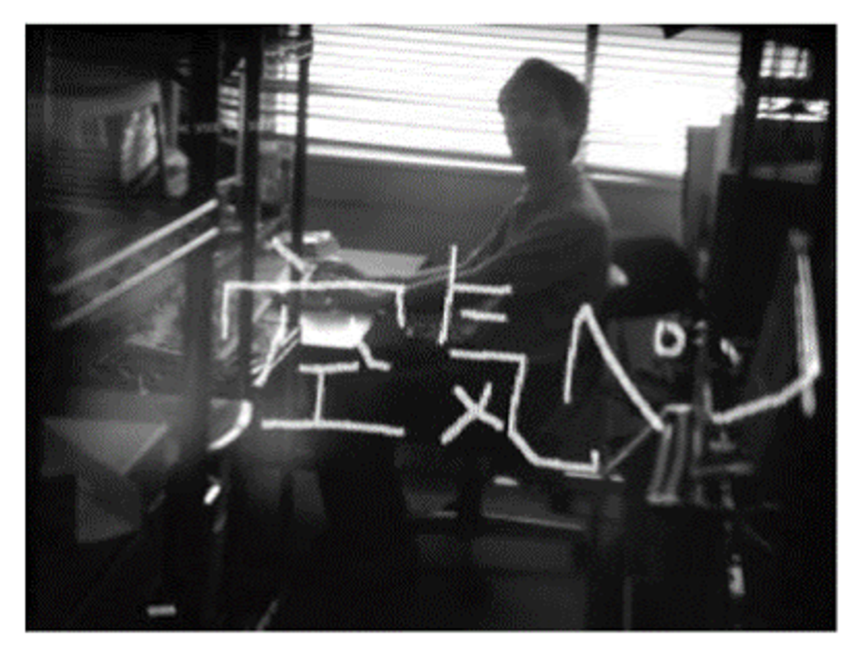
\includegraphics[clip,height=5.0cm,width=6.0cm]{./tegakijouhou.eps}
    \caption{描いた情報}
    \label{fig:tegakijouhou}
  \end{center}
\end{figure}

\begin{figure}[H]
  \begin{center}
    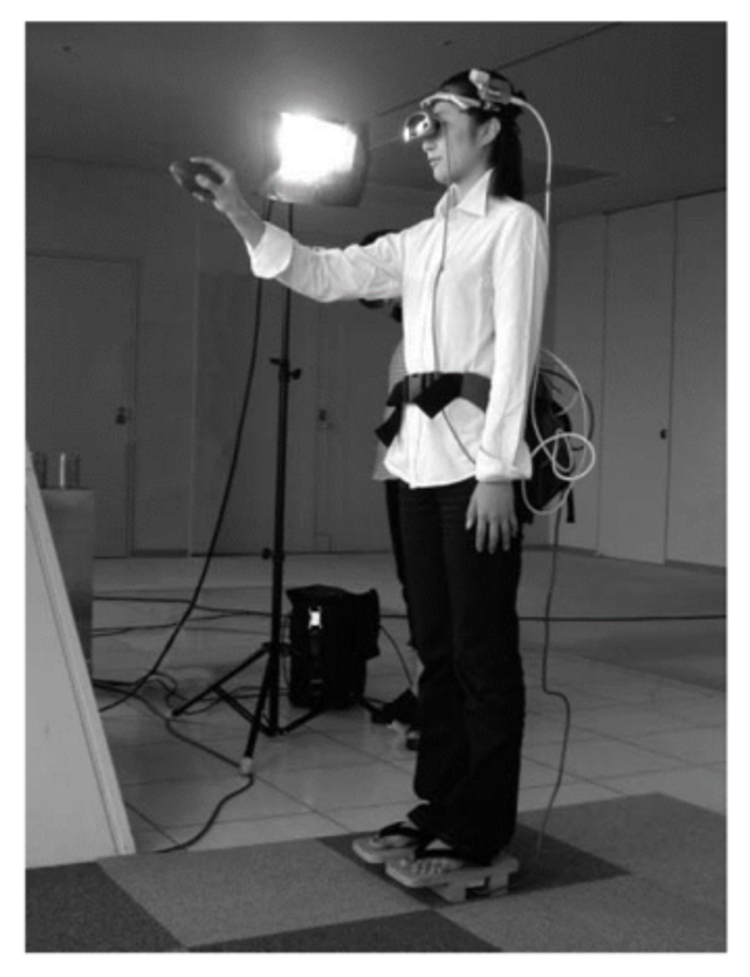
\includegraphics[clip,height=7.0cm,width=6.0cm]{./kuukipen.eps}
    \caption{空気ペン}
    \label{fig:kuukipen}
  \end{center}
\end{figure}

また、近年の研究ではSunら\cite{sun}は携帯端末からのWi-Fi信号を利用してハンズフリーでの描画を可能にするWiDrawを作成した。従来の研究では、ユーザーがワイヤレストランスミッタを保持する必要があるか、カスタムワイヤレスハードウェアを必要とするか、事前定義されたハンドジェスチャのみを決定する必要があったが、この研究ではウェアラブルデバイスを必要としない、W-iFiカードを使用した初めてのモーショントラッキングシステムを開発した(図\ref{fig:widraw})。

\begin{figure}[H]
  \begin{center}
    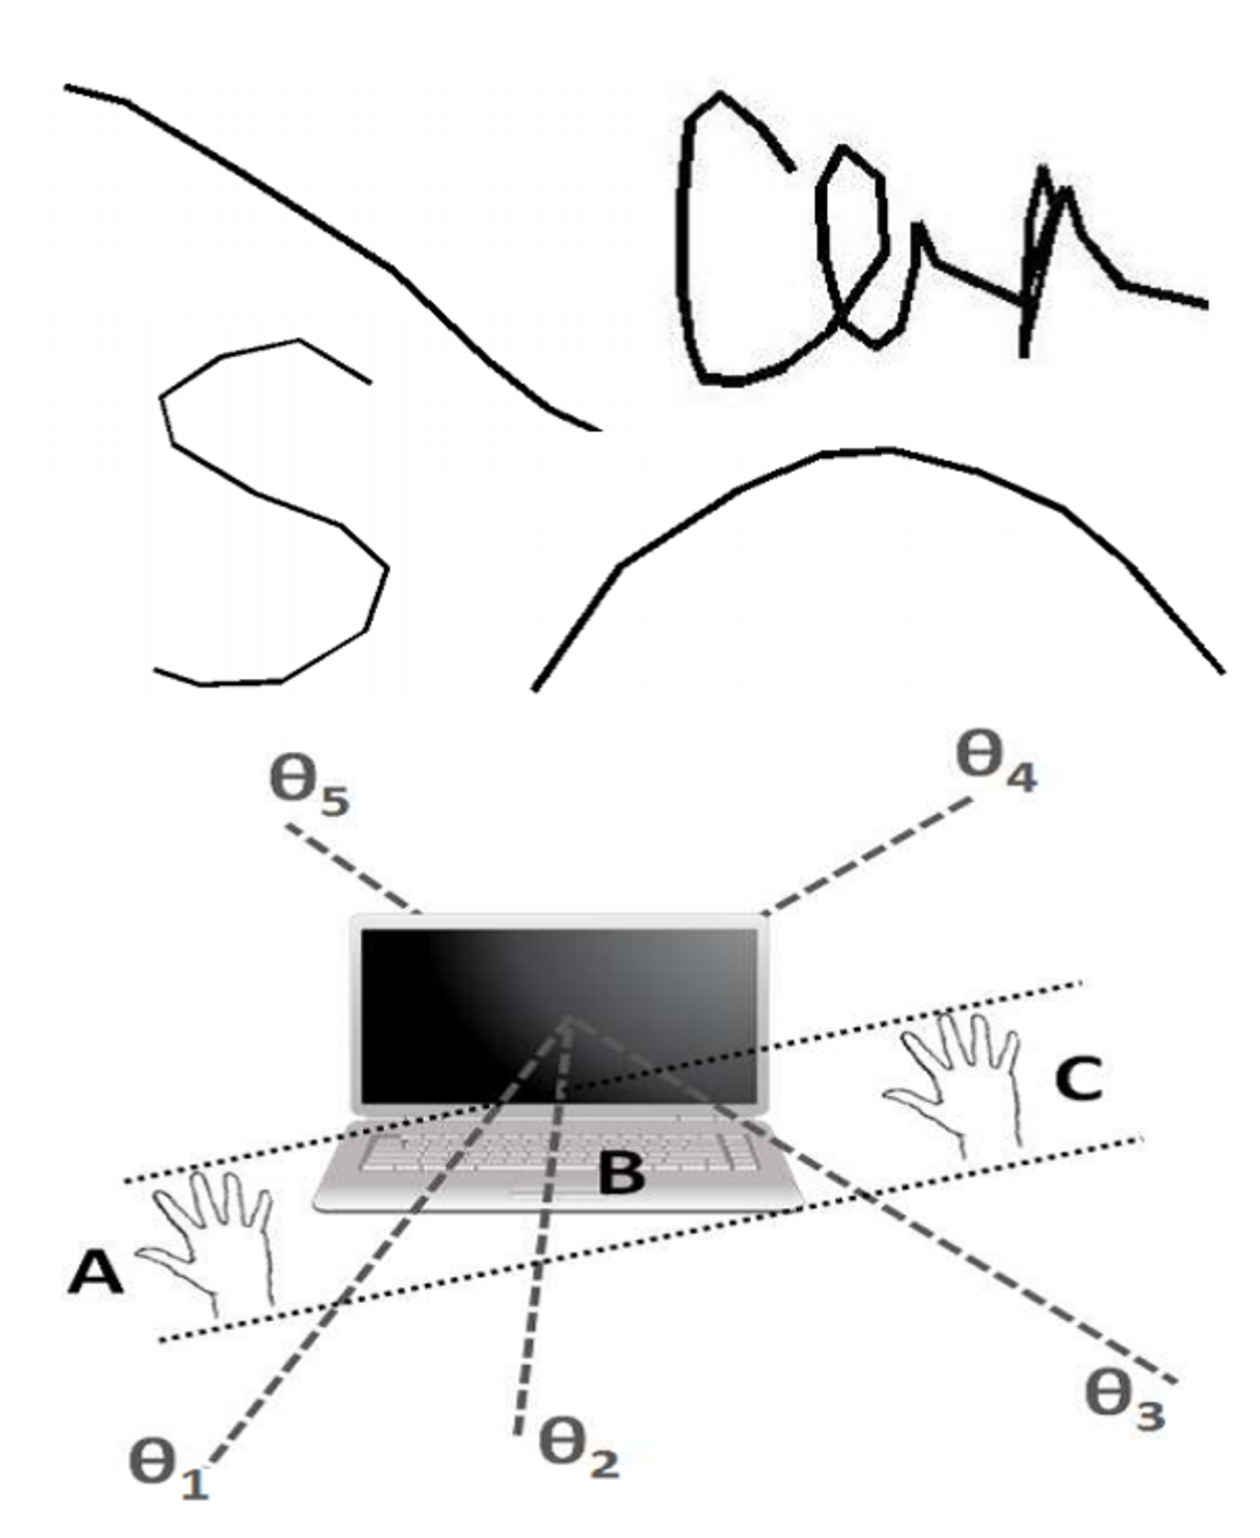
\includegraphics[clip,height=7.0cm,width=6.0cm]{./widraw.eps}
    \caption{WiDraw}
    \label{fig:widraw}
  \end{center}
\end{figure}


\subsubsection{実世界の物に関連付けてアイデアを残す研究}
高山ら\cite{tano},\cite{tano2}は実世界のどのような時間・場所であっても、ユーザが思い浮かんだふとしたアイデアを、生起を誘発したコンテキストに対応付けて保存し、それを他のユーザと共有できるシステムを作成した(図\ref{fig:informal}, \ref{fig:informal2})。ユーザーは同じような状況の時にコンテキストに対応づけて保存したインフォーマル情報を見ることができるようになった。多くのユーザーが思い浮かんだインフォーマル情報を保存することによって、実世界自体が巨大な掲示板のようになり、これによってユーザは状況に合った質の良い情報を得ることが可能になった。

\begin{figure}[H]
  \begin{center}
    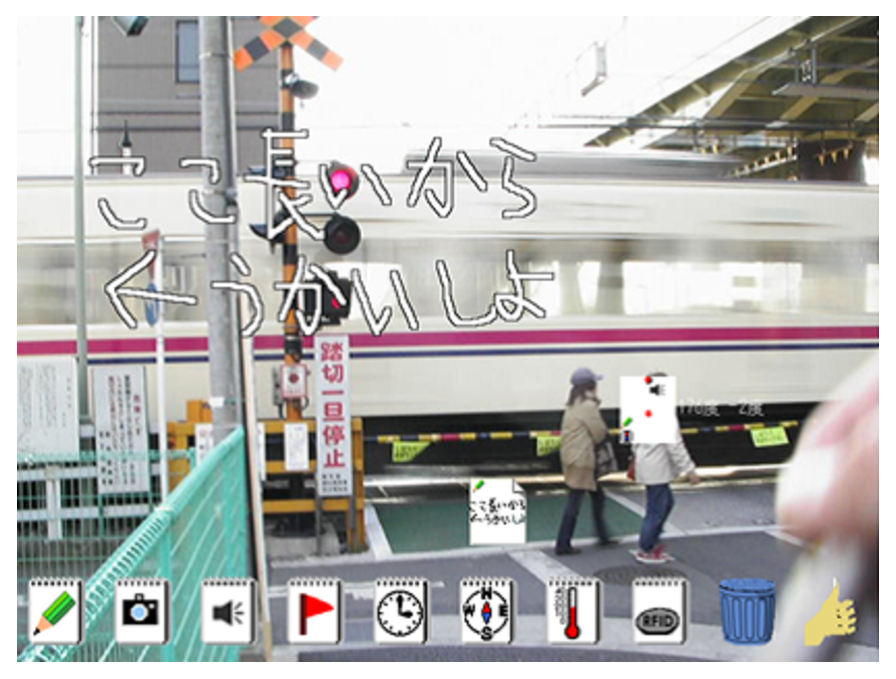
\includegraphics[clip,height=5.0cm,width=6.0cm]{./informal.eps}
    \caption{実世界の場所に関連付けてアイデアを保存}
    \label{fig:informal}
  \end{center}
\end{figure}

\begin{figure}[H]
  \begin{center}
    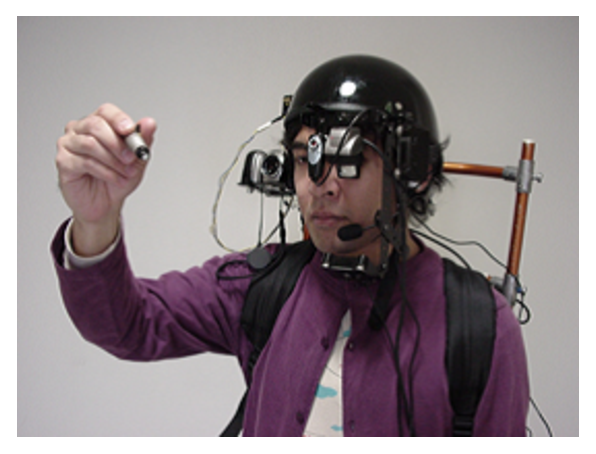
\includegraphics[clip,height=5.0cm,width=7.0cm]{./informal2.eps}
    \caption{機器を装着してるときの様子}
    \label{fig:informal2}
  \end{center}
\end{figure}

近年の研究では吉野ら\cite{yoshino}は実世界の物と関連付けたアイデアの共有による発想支援システム「ものぴこん」の開発をした。創造能力低下の原因として、日常生活における継続的な創造的思考の機会の減少が挙げられていた。この研究では、人は実空間上の「もの」を見ることで視覚刺激を受け、新しいアイデアを発想できるということに着目した。そこで、特定物体認識技術を用いることで、身の周りの「もの」を介してアイデアを日常的に共有するシステム「ものぴこん」の開発を行った(図\ref{fig:monopikon})。

\begin{figure}[H]
  \begin{center}
    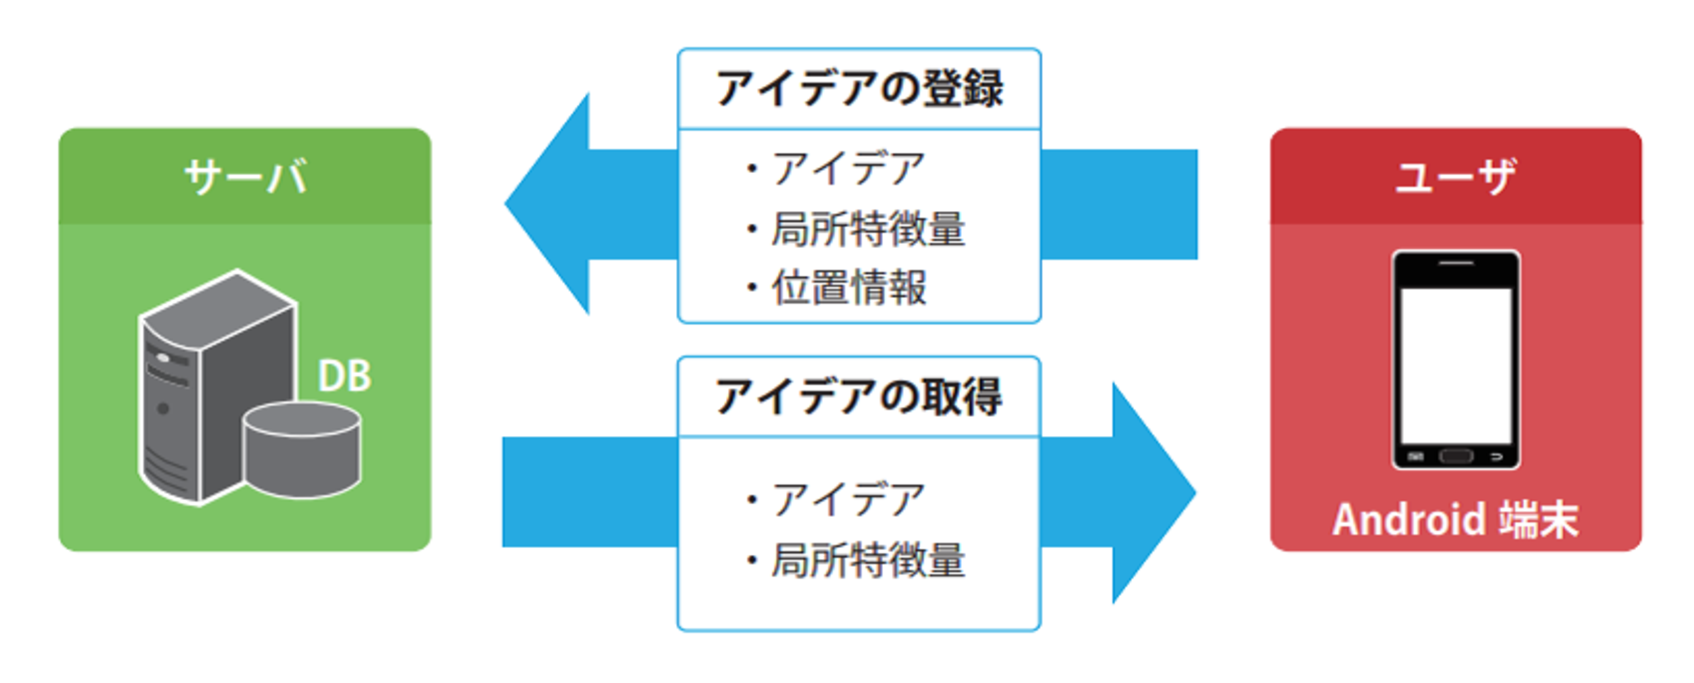
\includegraphics[clip,height=4.0cm,width=8.0cm]{./monopikon.eps}
    \caption{ものぴこんのシステム構成}
    \label{fig:monopikon}
  \end{center}
\end{figure}

\subsubsection{空間上に描いた情報を複数人に共有する研究}
長田ら\cite{nagata}はスマートグラスを用いた仮想空間への手書き情報共有システムを開発した(図\ref{fig:kasoukuukan})。ジェスチャの認識を用いて指の追跡を行い、軌跡を描くことで手書き情報を実現した。空間への描画は物体の動きをカメラで捉え行う。これによって仮想空間において手書き情報を共有することができるようになった。

\begin{figure}[H]
  \begin{center}
    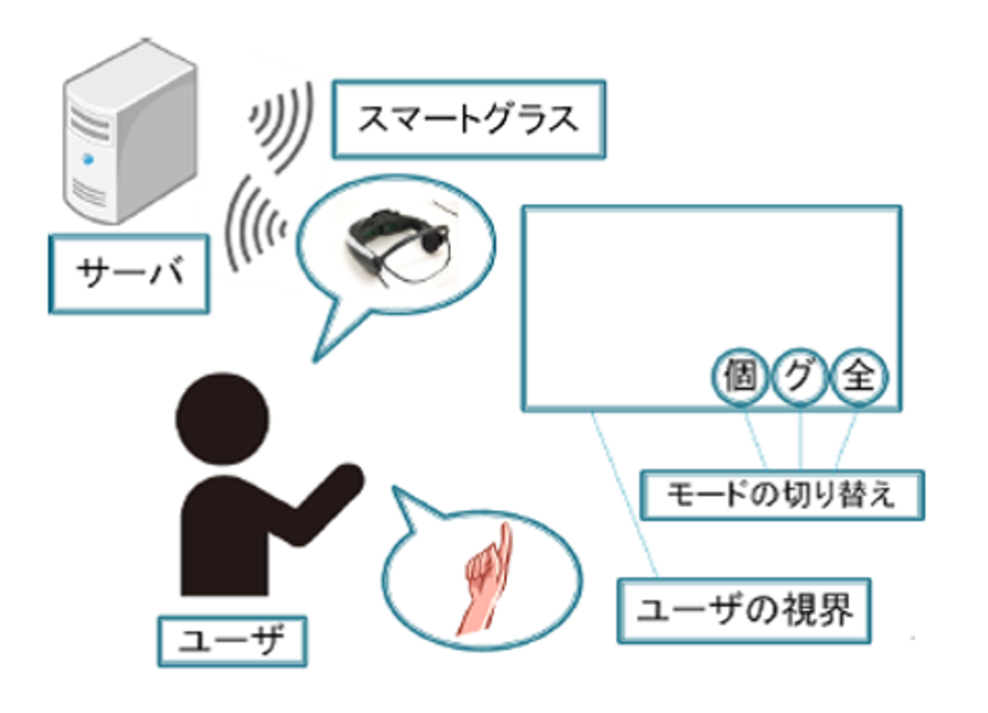
\includegraphics[clip,height=5.0cm,width=7.0cm]{./kasoukuukan.eps}
    \caption{仮想空間への情報共有システム}
    \label{fig:kasoukuukan}
  \end{center}
\end{figure}

\subsection{従来研究の問題点}

\newpage
\section{複数人で使用可能でどこでも利用できるシステムのコンセプト}
本章では、

\subsection{新しいシステムのコンセプトの提案}
従来研究では一人で使用をすることを想定していたり、使用できる場所が限定される、持ち運びが難しい、操作が複雑等の問題点があった。

アイデアは一人で深く考えて練ったり生み出すこともあるが、友人との話し合いをしたり、議論をしていくうちにアイデアが生まれることがある。よって複数人で使用できるシステムが必要である。

アイデアはふとしたときに突然思い浮かぶものである。現状、私達は浮かんだアイデアを紙に書き留めたり、PCを利用してメモを取っている。しかし、アイデアが思い浮かぶのは座って作業しているときだけとは限らない。外で歩いているときや、机やホワイトボード等がないような場面でも突然思い浮かぶことがある。したがって、場所を限定することなく、どこでも使用できるシステムが必要である。

思い浮かんだアイデアは短い言葉だけで表すことが難しい場合もある。また、話した内容もそのまま残しておきたい場合もある。また、人によって入力のしやすい方法は異なる。よって、複雑なジェスチャをすることなく直感的に様々な入力ができるようなシステムが必要である。

そこで、本研究は以下のようなシステムを提案する(図\ref{fig:concept})。

\begin{enumerate}[(1)]
 \item 複数人で話し合ってアイデアを生み出し、お互いのメモを共有することができる。
 \item 実世界の広い空間上の任意の場所にメモを置くことができ、どこでも場所を選ばず利用できる。
 \item 簡単な操作で直感的で様々な入力ができる。
\end{enumerate}

\begin{figure}[H]
  \begin{center}
    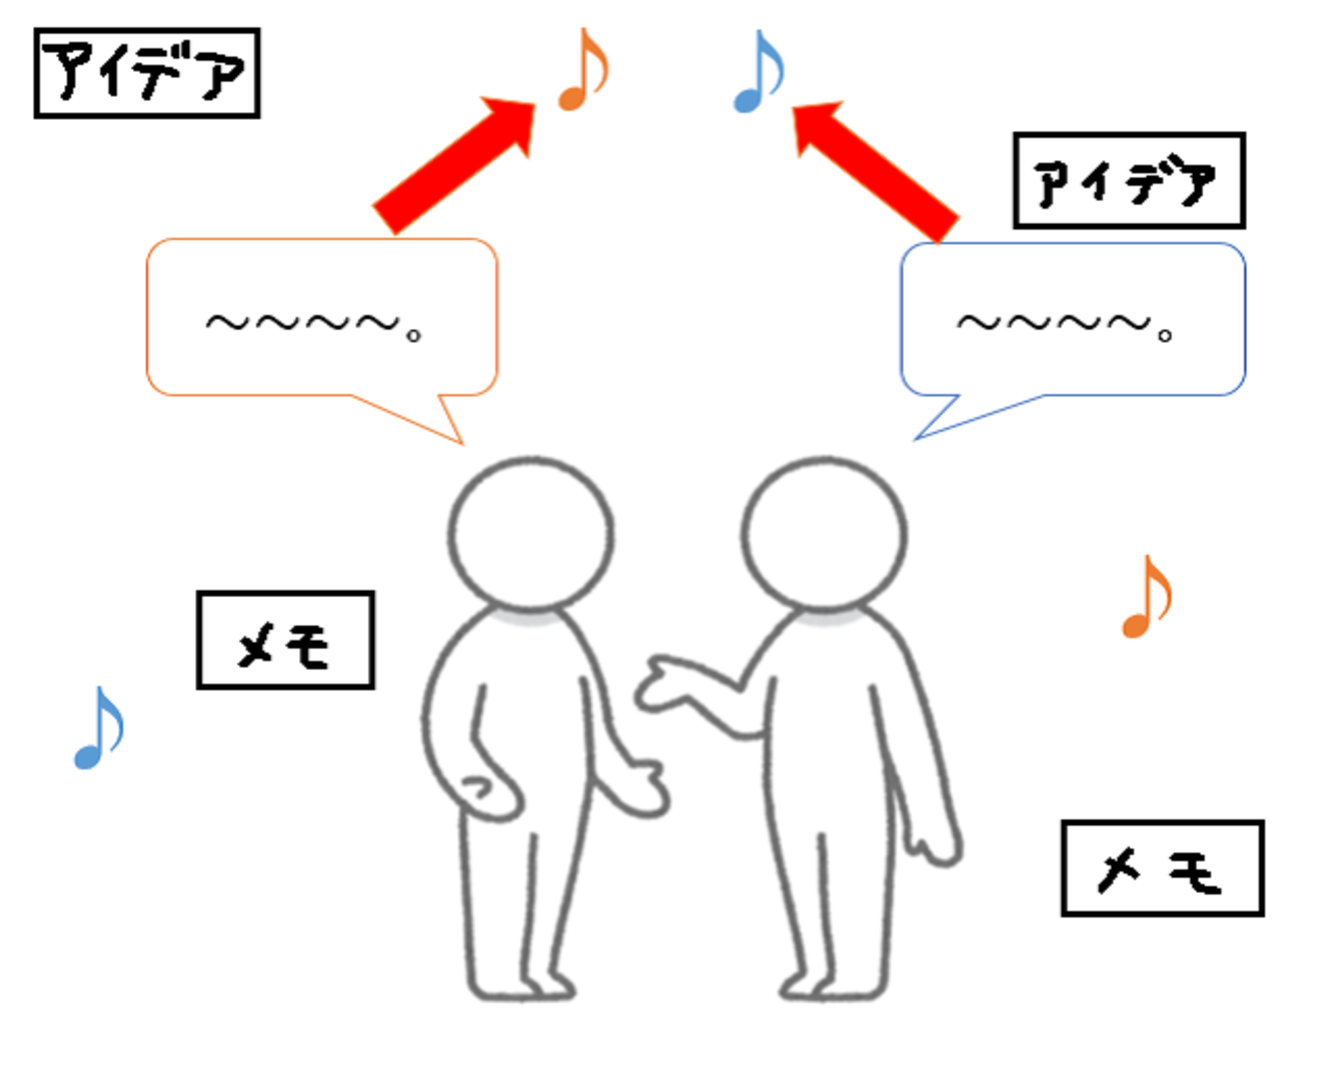
\includegraphics[clip,height=5.0cm,width=6.0cm]{./concept.eps}
    \caption{本研究のコンセプト}
    \label{fig:concept}
  \end{center}
\end{figure}

\subsection{利用シーン}

\subsection{様々なアイデアの形}
アイデアの形は様々である。大きく分けると描いて残すアイデアと話して残すアイデアがあるが、それぞれのアイデアも様々な形がある。以下ではそれぞれのアイデアを細かく分けて分類した上でそれぞれについて詳しく説明する。

\subsubsection{描いて残すアイデア} \label{draw_idea}
描いて残すアイデアを細かく分けると図\ref{fig:draw_idea}のようになる。描いて残すアイデアは、最初に絵と文字に分けることができると考えられる。更に絵のアイデアは、立方体等のように空間上に線を引いて描く3Dのアイデアと、空間上に仮想的な平面を用意してそこに丸や四角形等のように平面上に線を引いて描く2Dのアイデアに分けることができると考えられる。また、文字のアイデアも同様に立体的な形を持つ3Dのアイデアと、平面上に描いて残す2Dのアイデアに分けることができると考えられる。この2Dの文字の文字に関しては実際に空間上に描いて残すには問題がある。この問題点に関しては次章で詳しく述べる。

\begin{figure}[H]
  \begin{center}
    \includegraphics[clip,height=7.0cm,width=8.0cm]{./draw_idea.eps}
    \caption{描いて残すアイデアを分類}
    \label{fig:draw_idea}
  \end{center}
\end{figure}

\subsubsection{話して残すアイデア} \label{speak_idea}
話して残すアイデアを細かく分けると図\ref{fig:speak_idea}のようになる。話して残すアイデアは、最初に絵と文字と感嘆詞に分けることができると考えられる。更に絵のアイデアは、「立方体」と発声して立方体等を出現させて残す3Dのアイデアと、「四角形」と発声して平面の形をとった四角形等を出現させて残すアイデアがあると考えられる。また、文字のアイデアは視覚的に見ることができるテキスト形式のアイデアと、議事録のように話した内容をそのままを音声として残すバイナリ形式のアイデアに分けることができると考えられる。テキスト形式の文字のアイデアは実際に空間上に話して残すには問題がある。この問題点に関しては次章で詳しく述べる。最後に感嘆詞についてであるが、人は考える際には「うーん」や「えーっと」等、思わず声に出してしまうことがある。また、声に出すことだけに限らず、頭を傾げたり、頷いたりすることもある。これらは一人で考える際には重要ではないが、複数人で話し合ってアイデアを出すときには相手がどう考えているかがある程度わかる可能性があると考えられる。

\begin{figure}[H]
  \begin{center}
    \includegraphics[clip,height=7.0cm,width=8.0cm]{./speak_idea.eps}
    \caption{話して残すアイデアを分類}
    \label{fig:speak_idea}
  \end{center}
\end{figure}

\newpage
\section{システム設計}
本章ではまず前章で述べた(1)、(2)、(3)を踏まえた上でシステムの全体構成について述べる。その次にそれぞれの機能の設計に関して詳しく説明する。また、ハードウェアは可搬性を考慮して、マイクロソフト社のHoloLens\cite{hololens}を使用する。

\subsection{全体構成}
(1)複数人で話し合って実世界の3D空間上に残したお互いのメモを共有する機能を実現するために、サーバを介して空間を共有する機能が必要である。(2)実世界の広い空間上に任意の場所にメモを置く際には、遠くにあるメモに対して操作する機能が必要である。また、(3)簡単な操作で直感的な様々な入力を可能にするには、3D空間上に描画する機能だけではなく、マルチモーダルな入力が必要となる。以上より、システムの機能としては大きく分けて、メモを入力、メモを操作、メモを共有の三つであり、以下に詳細を述べる(図\ref{fig:system_zentai})。

\begin{figure}[H]
  \begin{center}
    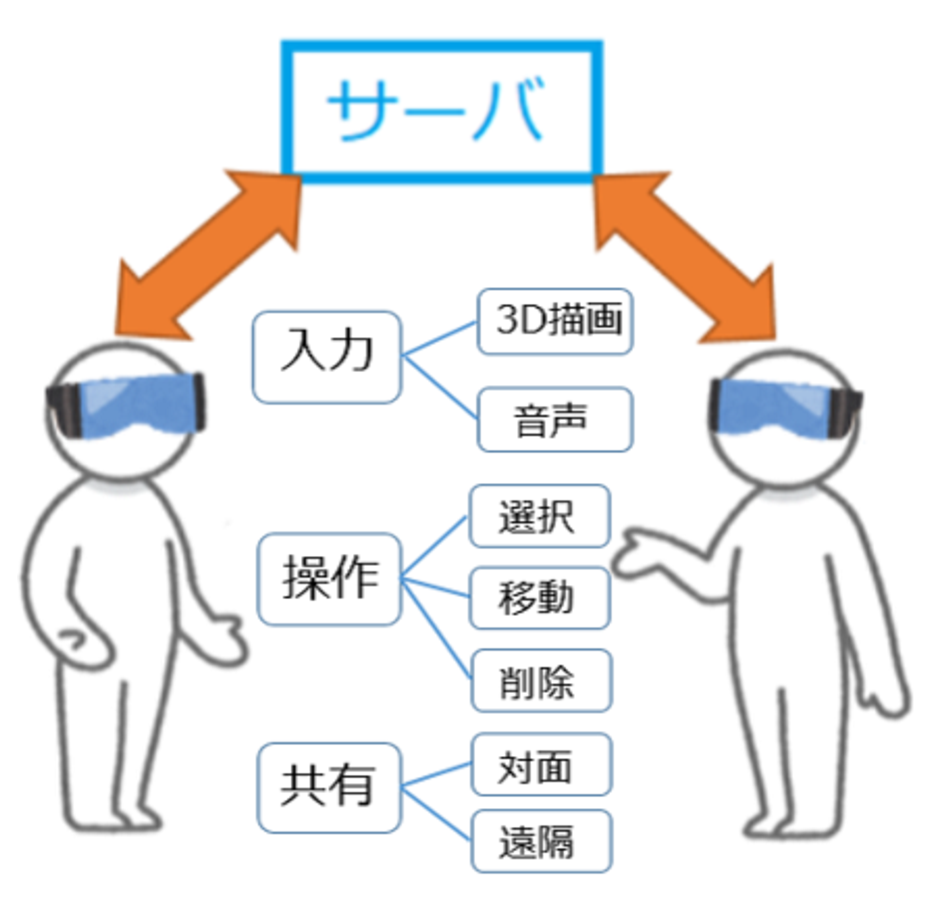
\includegraphics[clip,height=7.0cm,width=7.0cm]{./system_zentai.eps}
    \caption{システムの全体構成}
    \label{fig:system_zentai}
  \end{center}
\end{figure}

\subsection{メモを入力}

\subsubsection{描いて残すメモ}
\ref{draw_idea}より描いて残すアイデアは、最初に絵と文字に大きく分けることができることは述べた。まず、絵のメモをどうやって残すかについて詳しく説明する。3Dの絵に関しては、タップ&ホールドを使用して空間上に線を引いて描くようにする(図\ref{fig:3d_draw})。ここで言うタップとは空間上で人差し指と親指を一度つまんで離す動作のことであり、スマートフォンで言えば画面を指で一度タッチする動作のことである。ホールドは人差し指と親指をつまんだ状態を維持することである。ホールドをしている間のみ空間上に線が出るようにして、立体的な絵を描くことができるように実現する。

\begin{figure}[H]
  \begin{center}
    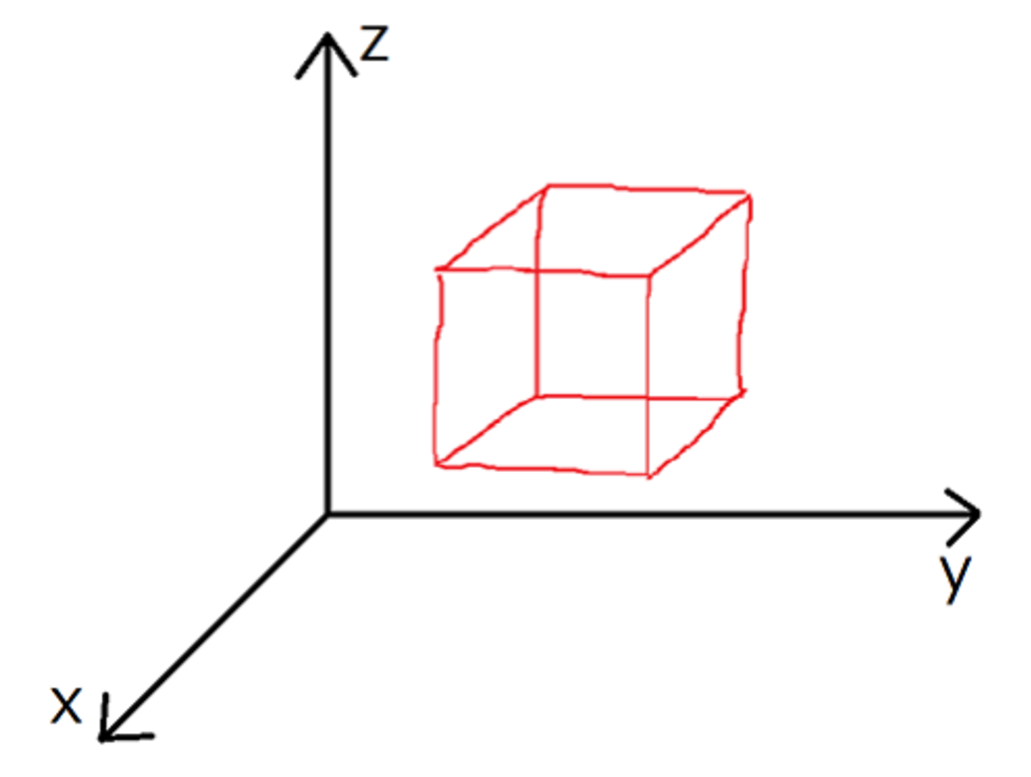
\includegraphics[clip,height=7.0cm,width=8.0cm]{./3d_draw.eps}
    \caption{3Dの絵のメモ}
    \label{fig:3d_draw}
  \end{center}
\end{figure}

2Dの絵に関しては、空間上に仮想平面を用意してその平面上に丸や四角形の図形等を描くようにする。

次に文字のメモをどうやって残すかについて説明をする。3Dの文字に関しては、3Dの絵と同様にタップ&ホールドを使用して空間上に線を引いて描くようにする(図\ref{fig:3d_moji})。

\begin{figure}[H]
  \begin{center}
    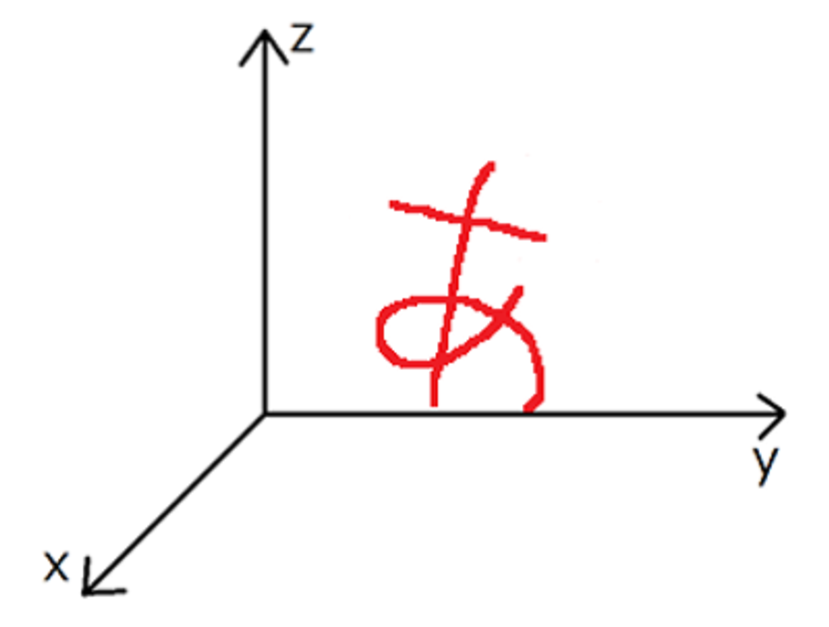
\includegraphics[clip,height=7.0cm,width=8.0cm]{./3d_moji.eps}
    \caption{3Dの文字のメモ}
    \label{fig:3d_moji}
  \end{center}
\end{figure}

2Dの文字に関しては、\ref{draw_idea}で述べたように空間上に2Dの文字を残すと見る方向によっては文字が見えないという問題が発生する。この問題の解決策としては、空間上に仮想平面を用意してその平面上に文字を書き、平面ごと相手の方向に向けるという方法を提案する(図\ref{fig:memo_kaiten})。

\begin{figure}[H]
  \begin{center}
    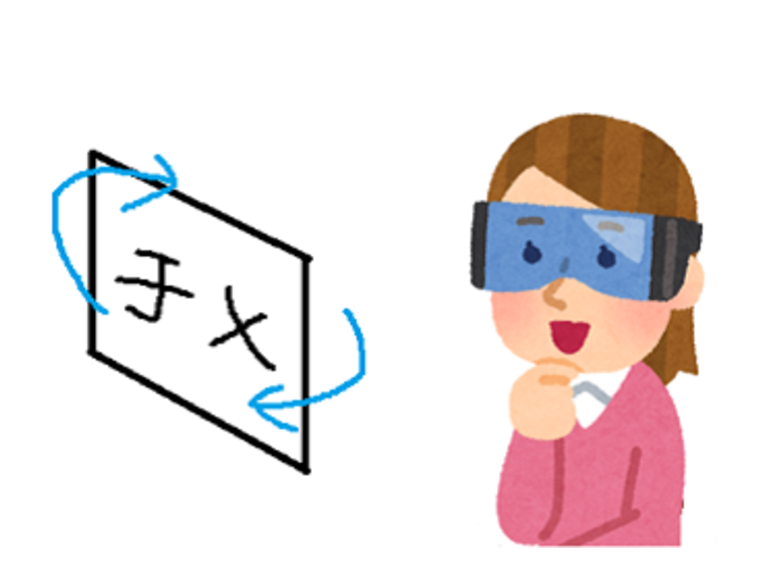
\includegraphics[clip,height=6.0cm,width=8.0cm]{./memo_kaiten.eps}
    \caption{空間上にある2Dの文字のメモは仮想平面ごと回転}
    \label{fig:memo_kaiten}
  \end{center}
\end{figure}

また、壁上やテーブル上等の平面のところに2Dの文字を残した場合、どうやって表示するかという新たな問題が挙がる。先ほどの空間上に残したメモの場合なら仮想平面をそのまま回転させて相手に向ければよいが、壁等にメモを残した場合は、そのまま回転させてしまうと壁の中に文字が隠れてしまう等の問題が発生する。この問題の解決策としては、壁等に残したメモはそのままにしておき、メモの内容のみを見やすいように自分や相手の目の前に表示するという方法を提案する(図\ref{fig:memo_wall})。

\begin{figure}[H]
  \begin{center}
    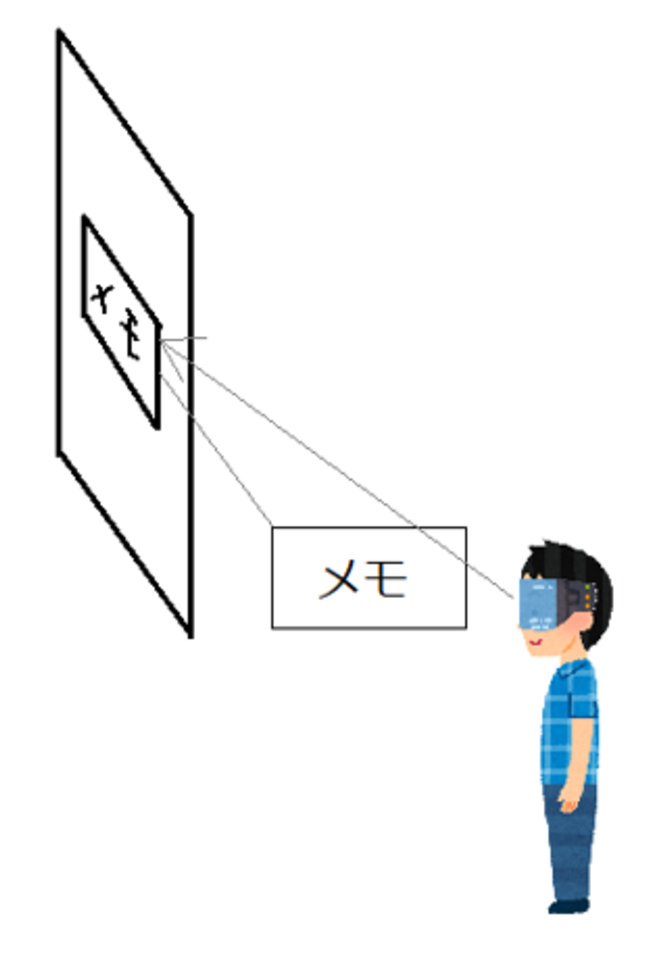
\includegraphics[clip,height=8.0cm,width=6.0cm]{./memo_wall.eps}
    \caption{壁等に残したメモは自分や相手の目の前に表示}
    \label{fig:memo_wall}
  \end{center}
\end{figure}

\subsubsection{話して残すメモ}


\subsection{メモを操作}


\subsection{メモを共有}


\newpage
\section{プロトタイプシステムの実装}
\subsection{はじめに}
この章では本研究で作成したシステム、FingCVについての評価実験を行う。最初に実験目的について述べ、その後に実験内容について詳しく説明をする。

\subsection{実験目的}
本実験により、FingCVを使用することによってスマートフォンの表示領域の広さを最大限生かすことができたかどうかについて評価をする。被験者には実験後、アンケートに回答してもらいFingCVの使用感についても評価をする。

\subsection{被験者情報}


\subsection{実験内容}


\subsection{アンケート内容}

\subsection{おわりに}
本章では本実験の目的、実験内容、アンケート内容について詳しく述べた。次章では実験で得られたタスク完了時間の結果やアンケート結果について詳しく述べる。

\newpage
\section{プロトタイプの評価実験}
\subsection{はじめに}
この章では本実験の測定結果やアンケート結果について詳しく述べる。それぞれの考察についても述べる。


\subsection{練習のべき乗則}


\subsection{測定結果}


\subsection{アンケート結果}
ここではアンケートの結果を示す。

\subsubsection{スクロールの精度}


\subsubsection{ズームの精度}


\subsubsection{疲労感の有無}



\subsubsection{スクロールやズームをしている際の画面全体の把握のしやすさ(タッチの場合)}



\subsubsection{スクロールやズームをしている際の画面全体の把握のしやすさ(FingCVの場合)}



\subsubsection{タッチ操作とFingCVの比較}


\subsubsection{総合的なFingCVの評価}


\subsubsection{追加してほしい機能}


\subsubsection{その他}


\subsection{おわりに}
本章では実験結果、アンケート結果について述べ、これらの結果についての考察を述べた。次章は本論文のまとめを述べ、今回の研究の改善すべき点や今後の展望について詳しく述べる。

\newpage
\section{実験結果と考察}
\subsection{まとめ}


\subsection{改善すべき点}


\subsection{展望}

\newpage
\section{おわりに}


\section*{謝辞}
本研究の全過程を通して多大なるご指導、ご鞭撻を賜りました電気通信大学大学院情報理工学研究科情報学専攻の田野俊一教授に心より深く感謝いたします。

また、本研究の遂行にあたり、有益なご助言とご鞭撻を頂きました橋山智訓准教授に厚く御礼申し上げます。

また、本研究の遂行にあたり、的確なご助言を頂きましたTIS株式会社の森真吾氏、井出将弘氏に深く感謝いたします。

最後に、研究活動や日々の研究室生活など様々な場面でお世話になりました、田野・橋山研究室の皆様に感謝申し上げます。

\newpage
\begin{thebibliography}{数字}
  \bibitem{memo} EvernoteやOneNote普及も…メモしない現代人の言い分; \textless\url{https://sirabee.com/2017/12/24/20161413693/}\textgreater2017年12月31日アクセス.
  \bibitem{hassouhou} 7つのアイデア発想フレームワーク; \textless\url{https://creive.me/archives/6722/}\textgreater2017年12月31日アクセス.
 \bibitem{siio} 山本, 椎尾: 空気ペン―空間への描画による情報共有―; 情報処理学会全国大会講演論文集, Vol.59, No.4,
pp.39-40(1999).
  \bibitem{siio2} 椎尾, 山本: コミュニケーションツールのための簡易型AR システム; コンピュータソフトウェア, Vol.19,
No.4, pp.246-253(2002).
  \bibitem{sun} Li Sun, Souvik Sen, Dimitrios Koutsonikolas, Kyu-Han Kim: WiDraw: Enabling Hands-free Drawing in the Air on Commodity WiFi Devices; Proceeding MobiCom '15 Proceedings of the 21st Annual International Conference on Mobile Computing and Networking, pp77-89(2015).
  \bibitem{tano} 高山, 瑞慶山, 田野, 岩田, 橋山: 実世界コンテキスト・情報を用いたユビキタスインフォーマルコミュニケーションの実装と評価; ヒューマンインタフェースシンポジウム2005, pp.955-958(2005).
  \bibitem{tano2} Tano, S., Takayama, T., Iwata, M. and Hashiyama, T.: Wearable Computer for Ubiquitous Informal Communication; Sixth International Workshop on Smart Appliances and Wearable Computing-IWSAWC 2006-(at 26th IEEE International Conference on Distributed Computing Systems
ICDCS), pp.1-8(2006).
  \bibitem{yoshino} 吉野, 松原: 実世界のモノと関連づけたアイデアの共有による発想支援システム「ものぴこん」の開発と評価, マルチメディア, 分散, 協調とモバイルシンポジウム(DICOMO2013), pp599-607(2013)
  \bibitem{nagata} 長田, 佐々木, 島田, 佐藤: スマートグラスを用いた仮想空間への手書き情報共有システム; 情報処理学会第77 回全国大会論文集, 3-205, 206(2015).
  \bibitem{hololens} Microsoft Inc: HoloLens; \textless\url{https://www.microsoft.com/ja-jp/hololens}\textgreater2018年1月2日アクセス.
\end{thebibliography}

\newpage
\section*{付録 本実験アンケート}
本実験後に回答してもらった各被験者のアンケート用紙を添付する。

\end{document}